\documentclass[tikz,border=4mm]{standalone}
      \usepackage{tikz}
      \usetikzlibrary{arrows.meta,positioning,calc,shapes.geometric}
      \begin{document}
      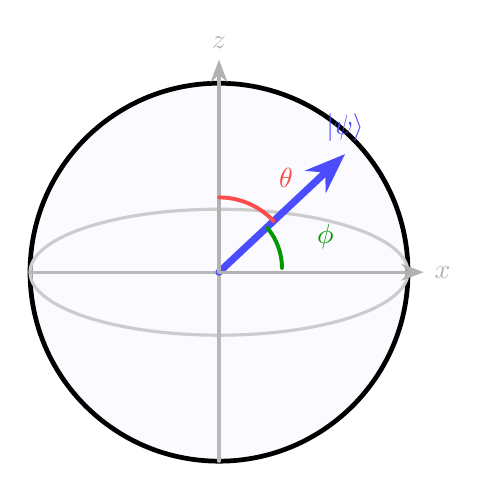
\begin{tikzpicture}[>=Stealth, line cap=round, line join=round]

\draw[fill=blue!2, line width=0.06cm] (6,4.5) circle (2.4);
\draw[gray!40, line width=0.04cm] (6,4.5) ellipse (2.4 and 0.8);
\draw[gray!55, line width=0.04cm] (3.6,4.5) -- (8.4,4.5);
\draw[gray!55, line width=0.04cm] (6,2.1) -- (6,6.9);
\draw[->, line width=0.09cm, blue!70] (6,4.5) -- (7.6,6.0) node[above] {$|\psi\rangle$};
\draw[->, line width=0.04cm, gray!60] (6,4.5) -- (8.6,4.5) node[right] {$x$};
\draw[->, line width=0.04cm, gray!60] (6,4.5) -- (6,7.2) node[above] {$z$};
\draw[red!70, line width=0.05cm] (6.0,5.45) arc[start angle=90,end angle=43,radius=0.95];
\node[red!70] at (6.85,5.7) {$\theta$};
\draw[green!60!black, line width=0.05cm] (6.8,4.55) arc[start angle=0,end angle=40,radius=0.8];
\node[green!60!black] at (7.35,4.95) {$\phi$};

      \end{tikzpicture}
      \end{document}
